\section{Zielsetzung}
Ziel des durchgeführten Versuchs ist es, Emissions- und Absorptionsspektren diverser Elemente aufzunehmen. Die verwendeten Wellenlängen liegen dabei im Bereich der Röntgenstrahlung.

\section{Theorie}
\label{sec:Theorie}
\subsection{Emission von Röntgenstrahlung}
Röntgenstrahlung entsteht beim Auftreffen von Elektronen auf eine Anode. Sie setzt sich aus der sogenannten Bremsstrahlung sowie der charakteristischen Röntgenstrahlung zusammen. Die Bremsstrahlung wiederum entsteht in Folge des Abbremsens der Elektronen im Coulombfeld des Atomkerns. Das Elektron verliert dabei kinetische Energie und das entstehende Photon wird mit eben dieser Energie ausgesandt. Dies führt zu einem kontinuierlichen Spektrum, dessen obere Begrenzung durch die maximale Energie des im elektrischen Feld beschleunigten Elektrons gegeben ist. Diese beträgt mit der Beschleunigungsspannung $U$
\begin{equation*}
  E_\text{acc} = eU \; .
\end{equation*}
Damit und mit der Energie eines Photons mit Wellenlänge $\lambda$
\begin{equation}
  E_\text{photon} = \frac{hc}{\lambda}
  \label{eq:Ephoton}
\end{equation}
ergibt sich die minimale Wellenlänge des durch Bremsstrahlung entstehenden Photons zu
\begin{equation}
  \label{eq:lambdamin}
  \lambda_\text{min} = \frac{hc}{eU} \; .
\end{equation}
Die charakteristische Strahlung hingegen entsteht durch Ionisierung des Anodenmaterials in Folge einschlagender Elektronen. Ein Elektron des Anodenmaterials verlässt daraufhin seine äußere Schale und wandert in die entstandene Leerstelle in der inneren Schale. Dabei wird Strahlung frei, dessen Energie der Differenz der beiden Energieniveaus entspricht. Die entstehenden Peaks sind dann charakteristisch für das jeweilige Anodenmaterial. Zur Benennung der für diesen Versuch relevanten Übergänge sowie der Visualisierung der Vorgänge dient Abbildung \ref{fig:transitions}.
\begin{figure}
  \centering
  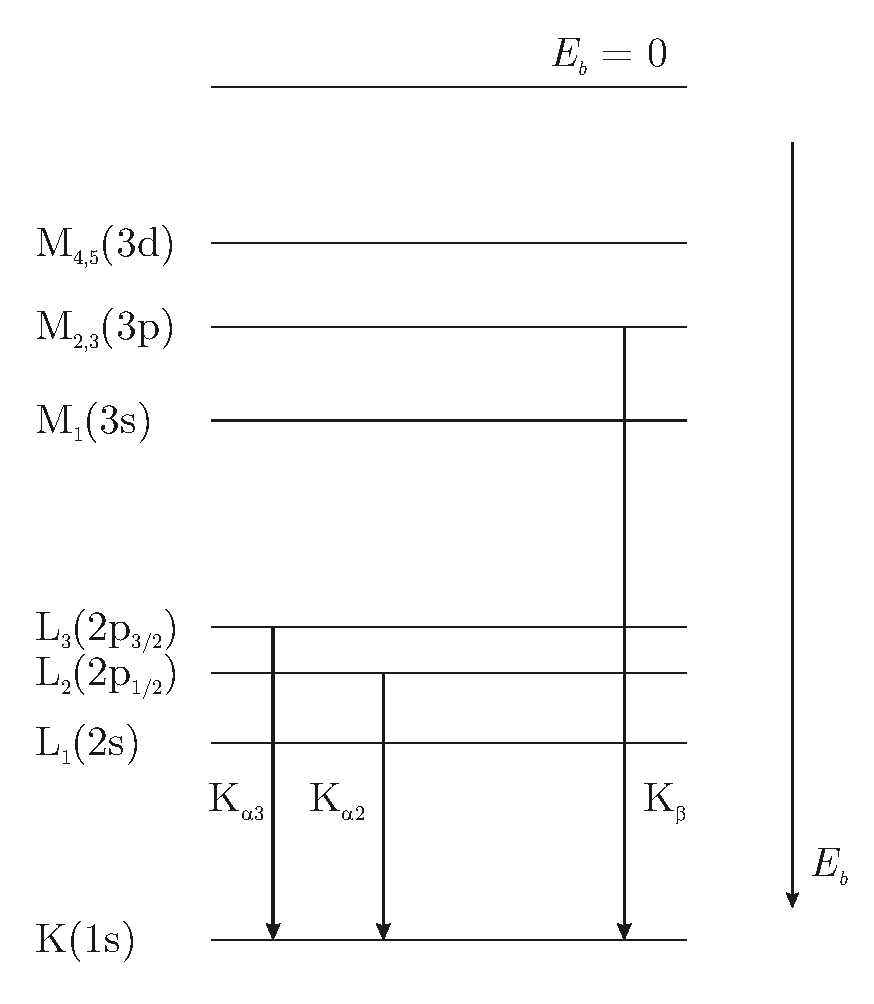
\includegraphics[width=0.5\textwidth]{ressources/transitions.pdf}
  \caption{Verschiedene Übergänge zwischen Energieniveaus und deren Bezeichnungen. Die Bindungsenergie nimmt nach unten hin zu. Während mehrere Energieniveaus aus derselben Schale, z.B. n=2, verschiedene Niveaus haben, lassen sich solche Übergänge nicht immer auflösen (Stichwort Feinstruktur).}
  \label{fig:transitions}
\end{figure}
Infolge von Bahndrehimpuls und Elektronenspin haben die Elektronen auch innerhalb einer Schale leicht unterschiedliche Bindungsenergien. Es ist also kein scharfer Peak zu erwarten, sondern vielmehr eine Superposition von mehreren Übergangsenergien. Dies wird als Feinstruktur bezeichnet.

\subsection{Absorption von Röntgenstrahlung}
Bei der Absorption von Röntgenstrahlung sind der Comptoneffekt sowie der Photoeffekt die maßgeblichen Vorgänge, die zur Abschwächung der Strahlung beitragen. Es zeigt sich, dass die Absorption in Abhängigkeit der Strahlung für verschiedene Absorbermaterialien charakteristische Verläufe annimmt. An den Übergangsenergien ist ein Sprung zu erwarten, sodass Strahlung höherer Energie stärker absorbiert wird. Dies ist dadurch zu begründen, dass nun die Energie ausreicht, solche Übergänge anzuregen. Diese Punkte im Spektrum werden als Kanten bezeichnet.

\subsection{Abschirmung}
Elektronen auf den äußeren Schalen werden durch Elektronen auf den inneren Schalen von der Kernladung abgeschirmt, sodass sie leichter zu ionisieren sind als die inneren Elektronen. Die äußeren Elektronen haben daher eine geringere Bindungsenergie. Das Moseleysche Gesetz beschreibt nun einen Zusammenhang zwischen Energie und Ordnungszahl. Dabei fließt die sogenannte Abschirmkonstante $\sigma$ ein.
\begin{equation}
  E_{nm} = Rhc(z-\sigma)²(\frac{1}{m²} - \frac{1}{n²})
\end{equation}
Hierin ist $R$ die Rydberg-Konstante, $h$ das Plancksche Wirkungsquantum, $c$ die Vakuumlichtgeschwindigkeit, $z$ die Kernladungszahl und $n$ und $m$ die Quantenzahlen der Schalen. Ein wichtiger Übergang ist der $K_\alpha$ Übergang. Hier ist $m=1$ und $n=2$, sodass für die Energie
\begin{equation}
  E_{21} = E_{K_\alpha} = Rhc (z-\sigma)²\frac{3}{4}
  \label{eq:sigma_k}
\end{equation}
folgt. Für Übergänge von höheren Schalen muss die Feinstruktur berücksichtigt werden, sodass die Berechnung der Abschirmkonstante kompliziert wird. Für die Übergänge der L-Kanten gilt jedoch folgende Gleichung \cite{skript}.
\begin{equation}
\sigma_\text{L} = Z - \sqrt{\frac{4}{\alpha} \sqrt{\frac{\Delta
      E}{h c R_\infty}} - \frac{5 \Delta E}{h c R}} \sqrt{ 1
  + \frac{19 \alpha ^2 \Delta E}{32h c R}}
\label{eq:sigma_l}
\end{equation}
Hierin sind $\alpha$ die Sommerfeldsche Feinstrukturkonstante und $\Delta_E$ die Energiedifferenz
\begin{equation}
  \Delta E = E_{L_{II}} - E_{L_{III}} \; .
\end{equation}

\subsection{Bragg-Bedingung}
Die Energie von Röntgenstrahlung kann mit Hilfe der Bragg-Bedingung gemessen werden. Fällt die Strahlung auf einen Kristall mit bekannter Gitterkonstante $d$, so erfährt die reflektierte Strahlung konstruktive Interferenz, wenn
\begin{equation}
  2d\sin(\Theta) = n \lambda
  \label{eq:bragg}
\end{equation}
gilt. Hierin sind $\Theta$ der Winkel zwischen Kristalloberfläche und eintreffender Strahlung, $\lambda$ die Wellenlänge der Strahlung und $n$ die Ordnungszahl. Durch Einsetzen von Gleichung \ref{eq:Ephoton} und Umstellen nach dem Winkel $\Theta$ folgt hieraus
\begin{equation}
  \Theta = \arcsin\left(\frac{nhc}{2dE}\right) \; .
  \label{eq:Theta}
\end{equation}
Falls $\Theta$ der Bragg-Bedingung \eqref{eq:bragg} genügt, wird dieser Winkel auch als Glanzwinkel bezeichnet, weil hier maximale Intensität zu erwarten ist. Für gleiche Ordnungszahl, z.B. $n=1$, gilt, dass der Glanzwinkel mit zunehmender Energie abnimmt.



% 2x2 Plot
% \begin{figure*}
%     \centering
%     \begin{subfigure}[b]{0.475\textwidth}
%         \centering
%         \includegraphics[width=\textwidth]{Abbildungen/Schaltung1.pdf}
%         \caption[]%
%         {{\small Schaltung 1.}}
%         \label{fig:Schaltung1}
%     \end{subfigure}
%     \hfill
%     \begin{subfigure}[b]{0.475\textwidth}
%         \centering
%         \includegraphics[width=\textwidth]{Abbildungen/Schaltung2.pdf}
%         \caption[]%
%         {{\small Schaltung 2.}}
%         \label{fig:Schaltung2}
%     \end{subfigure}
%     \vskip\baselineskip
%     \begin{subfigure}[b]{0.475\textwidth}
%         \centering
%         \includegraphics[width=\textwidth]{Abbildungen/Schaltung4.pdf}    % Zahlen vertauscht ... -.-
%         \caption[]%
%         {{\small Schaltung 3.}}
%         \label{fig:Schaltung3}
%     \end{subfigure}
%     \quad
%     \begin{subfigure}[b]{0.475\textwidth}
%         \centering
%         \includegraphics[width=\textwidth]{Abbildungen/Schaltung3.pdf}
%         \caption[]%
%         {{\small Schaltung 4.}}
%         \label{fig:Schaltung4}
%     \end{subfigure}
%     \caption[]
%     {Ersatzschaltbilder der verschiedenen Teilaufgaben.}
%     \label{fig:Schaltungen}
% \end{figure*}
